\documentclass[hyperref={pdfpagelabels=false},table,9pt,compress]{beamer}
% File Name: SetUp.tex
% Function: Make main settings of the document.


%%%%%%%%%%%%%%%%%%%%%%%%%%% BEGIN-Theme-settings %%%%%%%%%%%%%%%%%%%%%%%%%%
%%%%% http://www.hartwork.org/beamer-theme-matrix/
\usetheme{default} % Set the theme of the beamer.
%\usetheme{Frankfurt}                     %% Geovani style
%\setbeamercolor{alerted text}{fg=blue}   %% Geovani style
% W/o������:default, boxes, Bergen, Madrid, Pittsburgh, Rochester
% ���������:Antibes, JuanLesPins, Montpellier��
% ��Ŀ¼(TOC)�IJ�ߵ�����: Berkeley, PaloAlto, Goettingen, Marburg, Hannover��
% ��΢��frame������:Berlin, Ilmenau, Dresden, Darmstadt, Frankfurt, Singapore, Szeged��
% ����С�ڱ���: Copenhagen, Luebeck, Malmoe, Warsaw��
%\usecolortheme{default}  % Outer color themes. Alternatives: whale, seahorse, dolphin. default, beaver
\usecolortheme{orchid}  % Inner color themes. Alternatives: lily, orchid.
\useinnertheme[shadow]{rounded}
\usefonttheme{structurebold} % Font themes. Alternatives:  default, serif, structurebold, structureitalicserif, structuresmallcapsserif
\setbeamertemplate{frametitle}
{   \begin{center}
        \insertframetitle
    \end{center}
}
\setbeamertemplate{itemize items}[default] % Alternatives: default/triangle, circle, square, ball
\setbeamertemplate{enumerate items}[default] % Alternatives: default, circle, square, ball
\setbeamertemplate{navigation symbols}{}
\setbeamertemplate{footline}[frame number]
%\setbeamertemplate{footline}{%
%  \leavevmode%
%  \hbox{%
%    \begin{beamercolorbox}[wd=.333333\paperwidth,ht=2.25ex,dp=1ex,center]{author in head/foot}%
%      \usebeamerfont{author in head/foot}\insertshortauthor~(\insertshortinstitute)
%    \end{beamercolorbox}%
%    \begin{beamercolorbox}[wd=.333333\paperwidth,ht=2.25ex,dp=1ex,center]{title in head/foot}%
%      \usebeamerfont{title in head/foot}\insertshorttitle
%    \end{beamercolorbox}%
%    \begin{beamercolorbox}[wd=.333333\paperwidth,ht=2.25ex,dp=1ex,right]{date in head/foot}%
%      \usebeamerfont{date in head/foot}\insertshortdate{}\hspace*{2em}
%      \insertframenumber{} / \inserttotalframenumber \hspace*{2ex}
%    \end{beamercolorbox}
%    }%
%  \vskip0pt%
%}
%%%%%%%%%%%%%%%%%%%%%%%%%%%% END-Theme-settings %%%%%%%%%%%%%%%%%%%%%%%%%%%


%%%%%%%%%%%%%%%%%%%%%%%%%%%%%% BEGIN-Packages %%%%%%%%%%%%%%%%%%%%%%%%%%%%%
\usepackage{amsmath,amssymb,amsfonts}
\usepackage{mathrsfs}
\usepackage{color,xcolor}
\usepackage{graphicx,subfigure}
\usepackage{clock} % Use this package to insert a clock in the beamer.
\usepackage{textcomp}
\usepackage[T1]{fontenc}
\usepackage{verbatim}
\usepackage{moreverb}
\usepackage{multirow,multicol}
%\usepackage{url}
%\usepackage[colorlinks,linkcolor=blue,citecolor=blue,urlcolor=blue]{hyperref}%[colorlinks,linkcolor=blue,citecolor=blue,urlcolor=blue]
\usepackage{CJK}
%%%%%%%%%%%%%%%%%%%%%%%%%%%%%%%% END-Packages %%%%%%%%%%%%%%%%%%%%%%%%%%%%%


% \setbeamertemplate{navigation symbols}{} % Disable the buttons at the bottom.

\graphicspath{{Figures/}} % Set the directory where figures are saved.

%\AtBeginSection{
%  \begin{frame}{Outline}
%    \tableofcontents[currentsection,hideallsubsections]
%  \end{frame}
%}
%\AtBeginSubsection{
%  \begin{frame}{Outline}
%    \tableofcontents[currentsection,currentsubsection]
%  \end{frame}
%}
\AtBeginSection{
  \begin{frame}{Outline}
  \large{
  \tableofcontents[sections={\thesection}]  }
  \end{frame}
}

%%%%%%%%%%%%%%%%%%%% BEGIN-Theorem-like Environments %%%%%%%%%%%%%%%%%%%%%
\newtheorem{mybox}{}
\newtheorem{Con}{Conjecture}[section]
\newtheorem{Thm}{Theorem}[section]
\newtheorem{Prop}{Proposition}[Thm]
% show fig and table number
\setbeamertemplate{caption}[numbered]
% show theorems and example number
\setbeamertemplate{theorems}[numbered]
%%%%%%%%%%%%%%%%%%%%% END-Theorem-like Environments %%%%%%%%%%%%%%%%%%%%%%


%%%%%%%%%%%%%%%%%%%%%%%%%% BEGIN-New Commands %%%%%%%%%%%%%%%%%%%%%%%%%%%%
\newcommand{\email}[1]{Email: \href{mailto: #1}{\tt {\color{blue}#1}}}
\newcommand{\red}{\color{red}}
\newcommand{\blue}{\color{blue}}
\newcommand{\brown}{\color{brown}}
\newcommand{\orange}{\color{orange}}
\newcommand{\yellow}{\color{yellow}}
\newcommand{\Real}{\mathbb{R}}
\newcommand{\Tran}[1]{#1^\mathrm{T}}
\newcommand{\st}{\textnormal{s.t.}}
\newcommand{\dist}{\textnormal{dist}}
\newcommand{\bc}{\begin{center}}
\newcommand{\ec}{\end{center}}
\newcommand{\tbf}{\textbf}
\newcommand{\be}{\begin{equation}}
\newcommand{\ee}{\end{equation}}
\newcommand{\ba}{\begin{array}}
\newcommand{\ea}{\end{array}}
\newcommand{\btab}{\begin{table}\begin{tabular}}
\newcommand{\etab}{\end{tabular}\end{table}}
\newcommand{\nn}{\nonumber}
\newcommand{\xn}{x_1,x_2,\ldots,x_n}
\newcommand{\framee}[2]{\frame{\frametitle{#1} #2}}
\newcommand{\reff}[1]{(\ref{#1})} % ������
\newcommand{\inner}[2]{\left\langle#1,#2\right\rangle}

%\renewcommand{\baselinestretch}{1.3}
% Ĭ��������룬������ó����˶���
\renewcommand{\raggedright}{\leftskip=0pt \rightskip=0pt plus 0cm}
\raggedright
%\large
% define Roman numbers
\makeatletter
\newcommand{\rmnum}[1]{\romannumeral #1}
\newcommand{\Rmnum}[1]{\expandafter\@slowromancap\romannumeral #1@}
\makeatother
%%%%%%%%%%%%%%%%%%%%%%%%%%%% END-New Commands %%%%%%%%%%%%%%%%%%%%%%%%%%%%

\usepackage[ruled]{algorithm2e}

\begin{document}
\begin{CJK*}{GBK}{kai}

\title[distance geometry]{\textsc{A New Error Function and Its Application in Distance Geometry Problem}}
\author[Zhenli SHENG]{Zhenli Sheng (ʢ����)\\email: {\blue szl@lsec.cc.ac.cn}}
% \institute{Institute of Computational Mathematics and Scientific/Engineering Computing}
\institute[ICMSEC, CAS]{Institute of Computational Mathematics and Scientific/Engineering Computing,\\Chinese Academy of Sciences}
\date[]{joint work with {\blue Prof. Ya-xiang Yuan} \\\textrm{} \\January 8, 2013\\ seminar talk}
\frame{
\titlepage
}

% File Name: ThankYou.tex
% Function: Insert an Outline page.


%\section*{\textsc{Outline}}
%\begin{frame}
%\frametitle{\textsc{Outline}}
%\end{frame}

\begin{frame}
\frametitle{\textsc{Outline}}
\tableofcontents%[pausesections]
\end{frame}


\section{Problem Introduction}
\frame{
\frametitle{Distance Geometry Problem}
%Find the coordinate vectors $x_{1},x_{2},\ldots,x_{n}$ that satisfy several given distances among them. Mathematically, this problem can be stated as following, \\
\begin{block}{} %{Distance Geometry Problem}
Given an integer $d$, find $x_{1},x_{2},\ldots,x_{n} \in \Real^d$, such that
\begin{displaymath}
\|x_{i}-x_{j}\|=d_{ij},\quad (i,j) \in S.
\end{displaymath}
or
$$l_{ij}\leq \|x_i-x_j\|\leq u_{ij},\quad (i,j) \in S.$$
where $S$ is the given index set.
\end{block}

\begin{itemize}
  \item In general, it is a NP-hard problem.
  \item It has many applications:
   \begin{enumerate}[-]
     \item protein structure determination
     \item sensor network localization
     \item multidimensional scaling
     \item data mining: distance $\Leftrightarrow$ similarity
     \item ......
   \end{enumerate}
  \item In most of the applications, we have local and sparse distances.
\end{itemize}
}

\section{Various Error Functions}
\framee{How to Compare Different Models?}{
Usually, application problems may have several different models, a natural question is: {\blue which model is the best}? \pause
\begin{itemize}
  \item How to define goodness?
  $$ RMSD(X,Y) = \min_{Q,T}\{ \|X-YQ-T\|_{F}/\sqrt{n}: \Tran{Q}Q=I\} $$
  \item result = model + algorithm
\end{itemize}
\textrm{}\\[3mm] \pause
In our case, some possible ways:
\begin{itemize}
  \item Smoothness
  \item Number of "local minimizer"
  \item Numerical tests on the same instances
\end{itemize}
}


\begin{frame}[fragile]
\frametitle{Numerical Tools}
\begin{itemize}
  \item Ipopt ((\textbf{I}nterior \textbf{P}oint \textbf{OPT}imizer) is a software package for large-scale nonlinear optimization. It is designed to find (local) solutions of mathematical optimization problems of the form
      \be\begin{array}{cl} \min\limits_{x\in \Real^n} & f(x) \\ \st & g_L \leq g(x) \leq g_U\\ & x_L \leq x \leq x_U\end{array}\ee
      where $f(x)$ and $g(x)$ should be {\blue twice continuously differentiable}. %\\[2mm]
  \item AMPL: A Modeling Language for Mathematical Programming. They can provide first-order and second-order information via {\blue automatic differential}.
  \footnotesize{
  \begin{verbatim}
   param n;
   set Vertex := {1..n};
   set Edge within Vertex cross Vertex;
   param Dist {Edge} >= 0;
   param startvar {1..n,1..3};
   var x {1..n,1..3};
   minimize Smoothed_Stress_function:
      sum{(i,j)in Edge} ((x[i,1]-x[j,1])^2 + (x[i,2]-x[j,2])^2 +
   (x[i,3]-x[j,3])^2 - Dist[i,j]^2)^2;
  \end{verbatim}
  }
\end{itemize}
\end{frame}


\framee{Error Functions}{
\begin{itemize}
  \item Stress function
  $$Stress(\xn) = \sum_{(i,j)\in S} (\|x_i-x_j\|-d_{ij})^{2}$$
  \item Smoothed Stress function
  $$SStress(\xn) = \sum_{(i,j)\in S} (\|x_i-x_j\|^2-d_{ij}^2)^{2}$$
  \item Absolute Error function
  $$AbsErr(\xn) = \sum_{(i,j)\in S} \left|\|x_i-x_j\|^2-d_{ij}^2
  \right|$$
\end{itemize}
}

\framee{Stress VS SStress}{
\begin{itemize}
  \item $SStress$ is smoother, thus converges fast
  \be \frac{\partial Stress}{\partial x_i}=\sum_{j\in N(i)} 2(1-\frac{d_{ij}}{\|x_i-x_j\|})(x_i-x_j)\ee
  \be \frac{\partial SStress}{\partial x_i}=\sum_{j\in N(i)} 4(\|x_i-x_j\|^2-d_{ij}^2)(x_i-x_j)\ee
  \item Numerical tests: 100 random points in $[0,1]^3$, with different cutoffs, noiseless, random initial point.
      \btab{cc|ccc|ccc} \hline
      \multirow{2}*{cutoff} & \multirow{2}*{per} & \multicolumn{3}{c|}{SStress} & \multicolumn{3}{c}{Stress} \\ \cline{3-8}
      & & iter & time\footnote{ipopt} & RMSD  & iter & time & RMSD \\ \hline
        2 & 100  & 20 & 0.42 & 5.15-03 & 22 & 0.47 & 5.14-03 \\ \hline
      0.9 & 83.8 & 20 & 0.44 & 5.09-03 & 62 & 1.33 & 5.04-03 \\ \hline
      0.8 & 71.6 & 16 & 0.31 & 5.17-03 & 60 & 1.10 & 4.87-03 \\ \hline
      0.7 & 57.9 & 25 & 0.34 & 3.36-01 & 73 & 1.29 & 5.28-03 \\ \hline
      0.6 & 43.1 & 34 & 0.37 & 2.59-01 & 43 & 0.53 & 2.59-01 \\ \hline
      0.65& 50.6 & 37 & 0.54 & 5.37-03 & 39 & 0.54 & 4.25-01 \\ \hline
      \etab
  \item We also have tested on some other random data and with different noise,  \\ {\blue it is very hard to say which model leads to better result, but $SStress$ converges faster}.
\end{itemize}
}

\framee{SStress VS AbsErr}{
\begin{itemize}
  \item $AbsErr$ is more robust with {\blue large outliers}.
  \begin{figure}
  \centering
  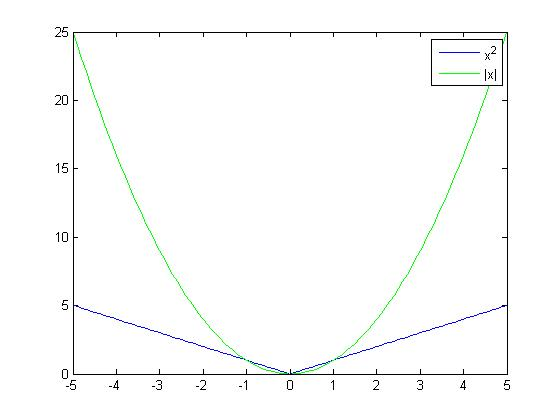
\includegraphics[width=0.4\textwidth]{abs.jpg}
  \end{figure}
  \item $SStress$ is twice continuously differentiable, while $AbsErr$ not. Therefore $SStress$ is used in direct error minimization.
  \item $AbsErr$ is widely used in SDP-based models with techniques as below,
      \begin{enumerate}[-]
        \item $\|x_i-x_j\|^2=e_{ij}^TYe_{ij}$, where $Y=X^TX.$
        \item $|x|=x_+-x_-$ with $x_+\geq 0, x_-\geq 0.$
      \end{enumerate}
\end{itemize}
}

\framee{Two New Error Functions}{
We construct the following two new error functions to measure the \textbf{Quo}tient \textbf{Err}ors, rather than difference errors,
$$QuoErr(\xn)=\sum_{(i,j)\in S} h(\frac{\|x_{i}-x_{j}\|^2}{d_{ij}^2})$$
where
$$h(x) = \left\{ \begin{array}{ll}
                \frac{1}{2}(x-1)^2 & \textrm{if } x\geq 1, \\
                x-1-log(x)         & \textrm{if } 0<x<1.
                \end{array} \right.
$$
or
$$h(x)= x-1-log(x) \quad \forall x>0.$$
Here, we choose the second function, the gradient can be calculated as
$$\frac{\partial QuoErr}{\partial x_i}=\sum_{j\in N(i)} (\frac{1}{d_{ij}^2}-\frac{1}{\|x_i-x_j\|^2})(x_i-x_j)$$
which is not continuous at $x_i=x_j$.
}

\framee{SStress VS QuoErr}{
\begin{itemize}
  \item Random intial point, noiseless
\btab{cc|ccc|ccc} \hline
      \multirow{2}*{cutoff} & \multirow{2}*{per} & \multicolumn{3}{c|}{SStress} & \multicolumn{3}{c}{QuoErr} \\ \cline{3-8}
      & & iter & time & RMSD  & iter & time & RMSD \\ \hline
        2 & 100  & 20 & 0.42 & 5.15-03 & 44 & 0.94 & 5.22-03 \\ \hline
      0.9 & 83.8 & 20 & 0.44 & 5.09-03 & 70 & 1.46 & 5.31-03 \\ \hline
      0.8 & 71.6 & 16 & 0.31 & 5.17-03 & 57 & 1.04 & 2.69-01 \\ \hline
      0.7 & 57.9 & 25 & 0.34 & 3.36-01 & 73 & 1.29 & 5.02-03 \\ \hline
      0.6 & 43.1 & 34 & 0.37 & 2.59-01 & 84 & 1.04 & 5.09-03 \\ \hline
      0.65& 50.6 & 37 & 0.54 & 5.37-03 & 85 & 1.17 & 5.49-02 \\ \hline
\etab
  \item Initial point: $X_{true}$*(1+0.5*(rand-0.5)*2), noise = 0.1
  \btab{cc|ccc|ccc} \hline
      \multirow{2}*{cutoff} & \multirow{2}*{per} & \multicolumn{3}{c|}{SStress} & \multicolumn{3}{c}{QuoErr} \\ \cline{3-8}
      & & iter & time & RMSD  & iter & time & RMSD \\ \hline
        2 & 100  & 8  & 0.15 & 3.48-02 & 13 & 0.29 & 1.81-02 \\ \hline
      0.9 & 83.8 & 8  & 0.16 & 3.29-02 & 21 & 0.45 & 1.86-02 \\ \hline
      0.8 & 71.6 & 8  & 0.18 & 2.93-02 & 15 & 0.27 & 1.93-02 \\ \hline
      0.7 & 57.9 & 10 & 0.15 & 3.00-02 & 23 & 0.35 & 2.20-02 \\ \hline
      0.6 & 43.2 & 16 & 0.20 & 2.89-02 & 21 & 0.25 & 2.17-02 \\ \hline
      0.5 & 28.8 & 10 & 0.08 & 3.25-02 & 28 & 0.23 & 2.58-02 \\ \hline
      0.4 & 16.4 & 16 & 0.07 & 3.99-02 & 48 & 0.21 & 6.57-02 \\ \hline
      0.3 &  7.6 & 45 & 0.10 & 1.66-01 & 39 & 0.09 & 1.62-02 \\ \hline
  \etab
  \item Usually, the QuoErr with not squared distance can get smaller RMSD error.
\end{itemize}
}

\framee{Short Summary}{
\begin{itemize}
  \item $SStress$ is fairly a good choice for postprocess procedure.
  \item $QuoErr$ provides better results when the distances are contaminated by noise, but it takes more time usually.
  \item In successful cases, we can get smaller objective function value than putting the true positions into these functions. \\
      $\Rightarrow$ If we expect better RMSD result, new model is needed.
  \item AbsErr is used in SDP based models.
  \item All of the models succeed or fail at the similar level.
\end{itemize}
}

\framee{Hessian Matrix}{
\footnotesize{
\begin{block}{Hessian Matrix of SStress}
Let $x=(x_{11},x_{12},x_{13},\ldots,x_{i1},x_{i2},x_{i3},\ldots,x_{n1},x_{n2},x_{n3})$, then the Hessian Matrix $\in \Real^{3n\times 3n}$ can be specified by
\begin{enumerate}[i)]
  \item \textbf{(diagonal item)} for $i=1:n, p=1:3$,
  \be\frac{\partial^2 SStress}{\partial^2 x_{ip}} = \sum_{j\in N(i)} 4\left(2(x_{ip}-x_{jp})^2+\|x_i-x_j\|^2-d_{ij}^2 \right) \ee
  \item \textbf{(nondiagonal item of diagonal block)} for $i=1:n,  p,q\in\{1,2,3\}$ with $p\neq q$,
  \be\frac{\partial^2 SStress}{\partial x_{ip}\partial x_{iq}} = \sum_{j\in N(i)} 8(x_{ip}-x_{jp})(x_{iq}-x_{jq}) \ee
  \item \textbf{(diagonal item of nondiagonal block)} for $i=1:n, k\in N(i), p=1:3$,
  \be\frac{\partial^2 SStress}{\partial x_{ip}\partial x_{kp}} = - 8(x_{ip}-x_{kp})^2-4(\|x_i-x_k\|^2-d_{ik}^2) \ee
  \item \textbf{(nondiagonal item of nondiagonal block)} for $i=1:n, k\in N(i), p,q\in\{1,2,3\}$ with $p\neq q$,
  \be \frac{\partial^2 SStress}{\partial x_{ip}\partial x_{kq}} = -8(x_{ip}-x_{kp})(x_{iq}-x_{kq}) \ee
  \item 0, otherwise.
\end{enumerate}
\end{block}
}
}

\framee{Picture of Hessian Matrix}{
\vskip-1cm
\huge{
$$\left( \begin{array}{ccccc}
\diamondsuit  &      &  \Box &      & \Box \\
      & \diamondsuit &       &      & \Box \\
\Box  &      &  \diamondsuit &      &      \\
\vdots&\vdots&       &\ddots&\vdots\\
\Box  & \Box &       &      & \diamondsuit \\
\end{array}\right)$$
}
\normalsize
\begin{itemize}
  \item Hessian is a sparse symmetric matrix.
  \item Each $\diamondsuit, \Box$ represents a $3\times3$ symmetric submatrix.
  \item The $(i,j)$-th block is zero matrix if $(i,j)\not\in S$.
  \item The diagonal $\diamondsuit$ is the negative sum of $\Box$ in the same row/column.
\end{itemize}
}

\framee{Regularization Term for Error Function}{
\begin{itemize}
  \item "The points estimated from these models tend to crowd together towards the center of the configuration. "\footnote{Biswas, P., Liang, T. C., Toh, K. C., Ye, Y., \& Wang, T. C. (2006). \emph{Semidefinite programming approaches for sensor network localization with noisy distance measurements}.}
      \begin{figure}
        \centering
        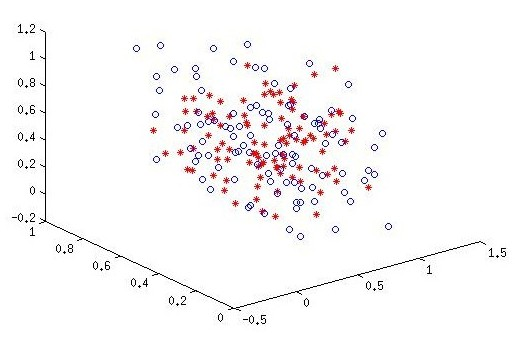
\includegraphics[width=0.45\textwidth]{bad2.jpg}\\
      \end{figure}
  \item They further proposed to add a regularization term to the objective function
      $$\lambda \sum_{i=1}^n\sum_{j=1}^n \|x_i-x_j\|^2$$
      However, it is very difficult to choose the parameter $\lambda$.
\end{itemize}
}

\section{Generalized DG Model and its SDP Relaxation}
\framee{Generalized DG Model}{
Sit and Wu (2011) \footnote{Sit, A., \& Wu, Z. (2011). \emph{Solving a generalized distance geometry problem for protein structure determination}. } proposed the following model to deal with distance bounds,
\be\label{model:1}
\begin{split}
  \max_{x_{i},r_{i}} \quad & \sum_{i=1}^{n} r_i \\
  \st                \quad & \|x_i-x_j\|+r_i+r_j\leq u_{i,j} \\
                           & \|x_i-x_j\|-r_i-r_j\geq l_{i,j}, \quad \forall (i,j)\in S\\
                           &  r_i\geq 0, \quad i=1,2,\ldots,n.
\end{split} \ee
where $x_i$ is the coordinate, $r_i$ is the fluctuation radius.
\begin{figure}
  \centering
  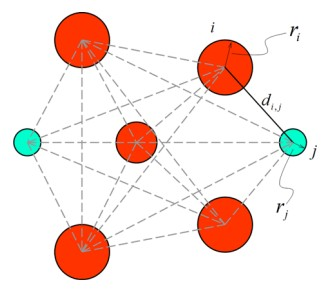
\includegraphics[width=0.45\textwidth]{GDG2.jpg}\\
\end{figure}
}

\framee{SDP Relaxation}{
Let $X=(x_1,x_2,\ldots,x_n)\in \Real^{3\times n}$ and $e_i$ be the $i$-th column of Identity matrix in appropriate dimensional space. Then, we have
\begin{equation}
\begin{split}
\|x_i-x_j\|^2 & = \|X(e_i-e_j)\|^2 \\
              & = e_{ij}^TX^TXe_{ij} \qquad (e_{ij}=e_i-e_j)
\end{split}
\end{equation}
Furthermore, let $R=(r_1,r_2,\ldots,r_n)\in \Real^{1\times n}$ be a row vector,
\begin{equation}
\begin{split}
(u_{ij}-r_i-r_j)^2 & = u_{ij}^2 - 2u_{ij}(r_i+r_j) + (r_i+r_j)^2 \\
                   & = u_{ij}^2 - 2u_{ij}R(e_i+e_j) + (R(e_i+e_j))^2 \\
                   & = u_{ij}^2 - 2u_{ij}Rf_{ij}+f_{ij}^TR^TRf_{ij} \qquad (f_{ij}=e_i+e_j )\\
                   & = u_{ij}^2 + \left\langle\left(\begin{array}{cc}
                   0 & -u_{ij}f_{ij}^T \\ -u_{ij}f_{ij} & f_{ij}f_{ij}^T \end{array}\right),\left(\begin{array}{cc}
                   1 & R \\ R^T & R^TR \end{array}\right)\right\rangle
\end{split}
\end{equation}
}

\framee{}{
To establish the associate SDP model, we let
$$Y=X^TX, \quad Z=\left(\begin{array}{cc} 1 & R \\ R^T & R^TR \end{array}\right),$$
and relax them to $Y\succeq0, Z\succeq0$. Therefore, by these notations, we can relax model (\ref{model:1}) to
\begin{equation}\label{model:SDP}
\begin{split}
  \min_{Y,Z} \quad & -\inner{\left(\begin{array}{cc}0&e^T/2\\e/2&0\end{array}\right)}{Z} \\
  \st        \quad & \inner{e_{ij}e_{ij}^T}{Y}+\inner{\left(\begin{array}{cc}0&-u_{ij}f_{ij}^T\\
  -u_{ij}f_{ij}&f_{ij}f_{ij}^T\end{array}\right)}{Z}\leq u_{ij}^2\\
  &\inner{e_{ij}e_{ij}^T}{Y}-\inner{\left(\begin{array}{cc}0&l_{ij}f_{ij}^T\\
  l_{ij}f_{ij}&f_{ij}f_{ij}^T\end{array}\right)}{Z}\geq l_{ij}^2, \quad \forall (i,j)\in S\\
  &\inner{\left(\begin{array}{cc}0&e_i^T/2\\e_i/2&0\end{array}\right)}{Z}\geq 0, \quad i=1,2,\dots,n \\
                           & \inner{e_1e_1^T}{Z}=1 \\
                           & Y\succeq 0, Z\succeq 0.
\end{split}
\end{equation}
}

%\framee{}{
%Currently, We would like to exploit the open solver \textbf{SDPT3} to solve this problem. Thus, model (\ref{model:SDP}) can be further reformulate as the standard form for SDPT3.
%\begin{equation}\label{model:SDPT3}
%\setlength\arraycolsep{3pt}
%%\setlength\arraylinesep{5pt}  % need package "tabls"
%\begin{array}{cccrcccl}
%  \min\limits_{Y,Z} \quad & && -\inner{\left(\begin{array}{cc}0&e^T/2\\e/2&0\end{array}\right)}{Z} &&&\\
%  \st        \quad & \inner{e_{ij}e_{ij}^T}{Y}&+&\inner{\left(\begin{array}{cc}0&-u_{ij}f_{ij}^T\\
%  -u_{ij}f_{ij}&f_{ij}f_{ij}^T\end{array}\right)}{Z}&+&\alpha_{ij}&=&u_{ij}^2\\
%  &\inner{e_{ij}e_{ij}^T}{Y}&-&\inner{\left(\begin{array}{cc}0&l_{ij}f_{ij}^T\\
%  l_{ij}f_{ij}&f_{ij}f_{ij}^T\end{array}\right)}{Z}&-&\beta_{ij}&=&l_{ij}^2, \quad \forall (i,j)\in S\\
%  & & &\inner{\left(\begin{array}{cc}0&e_i^T/2\\e_i/2&0\end{array}\right)}{Z}& +& t_i &= &0, \quad i=1,2,\dots,n \\
%  && &  \inner{e_1e_1^T}{Z}&&&=&1 \\
%  & \multicolumn{7}{l}{Y, Z\in K_s^{s_j},\quad \alpha_i, \beta_i, t_i \in K_l^{n_l}.}
%\end{array}
%\end{equation}
%}


\section{Ongoing works}
\frame{
\frametitle{Ongoing works}
\begin{itemize}
  \item Consider corresponding NSDP and ESDP model and facial reduction method to reduce the size of the problem.
  \item Exploit the extremely sparse structure of the SDP model to design a fast algorithm.
\end{itemize}
}


\frame{
%\frametitle{Q \& A}
\begin{center}
  \Large{  \textsc{Thank you for your attention!}}  \\
  \vspace{0.2cm}
  {\blue szl@lsec.cc.ac.cn }
\end{center}
}

\end{CJK*}
\end{document}
